\chapter{Application of Approach}

A proportion of the project time was spent researching reinforcement learning, in order to obtain the grounding required to design the environments, choose appropriate algorithms and implement them. Approximately three weeks were spent reading Sutton and Barto's `Introduction to Reinforcement Learning'\cite{Sutton:RLIntro01} cover to cover, and watching the DeepMind lecture series \cite{silver}. 

Next was designing the environment itself. An open source python library called OpenAI Gym was used to create the environments \cite{AIgym}. OpenAI Gym is a package that provides multiple pre-made environments to test reinforcement learning methods, but also allows for the creation of custom environments. By using gym we can ensure the environment's design is standardized to work in RL field, as well as use base functions within Gym, to make implementation faster. Nearly two weeks were spent learning the code base and learning how to use Gym, and two weeks were spent designing and implementing the different environments.

\begin{figure}[h]
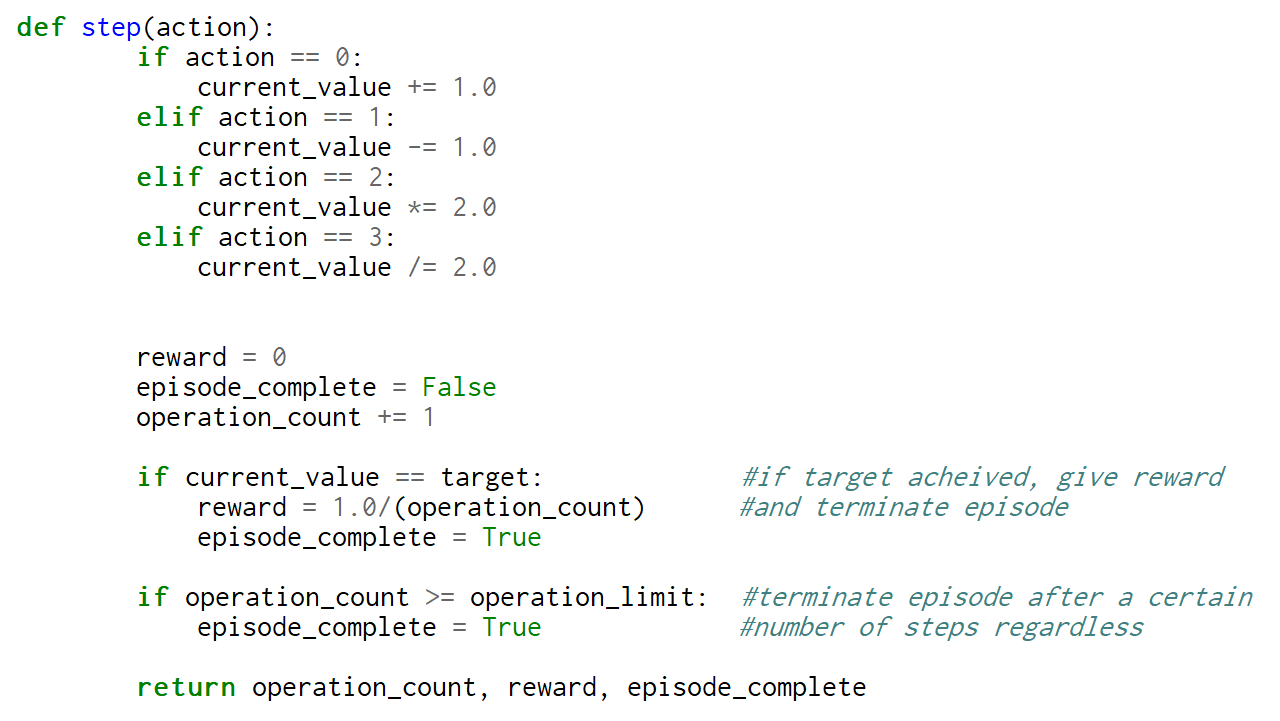
\includegraphics[width=\textwidth]{images/pseudo}
\caption[basic environment pseudocode]{pseudocode for the step function within the basic environment}
\label{fig:basicenv}
\end{figure}

Figure \ref{fig:basicenv} shows pseudocode of the step function for the most basic environment. Note that the possible actions are provided in the form of integers, 0 to 4. If the target is achieved or the limit of operations is hit the episode terminates. The reward is 0 if the target is not achieved, or a value of $1/n$, where $n$ is the number of operations taken to reach the target. The return is operation\_count (which is the state of the environment), the reward, and a boolean that determines whether or not the episode has terminated. 

\begin{figure}[h]
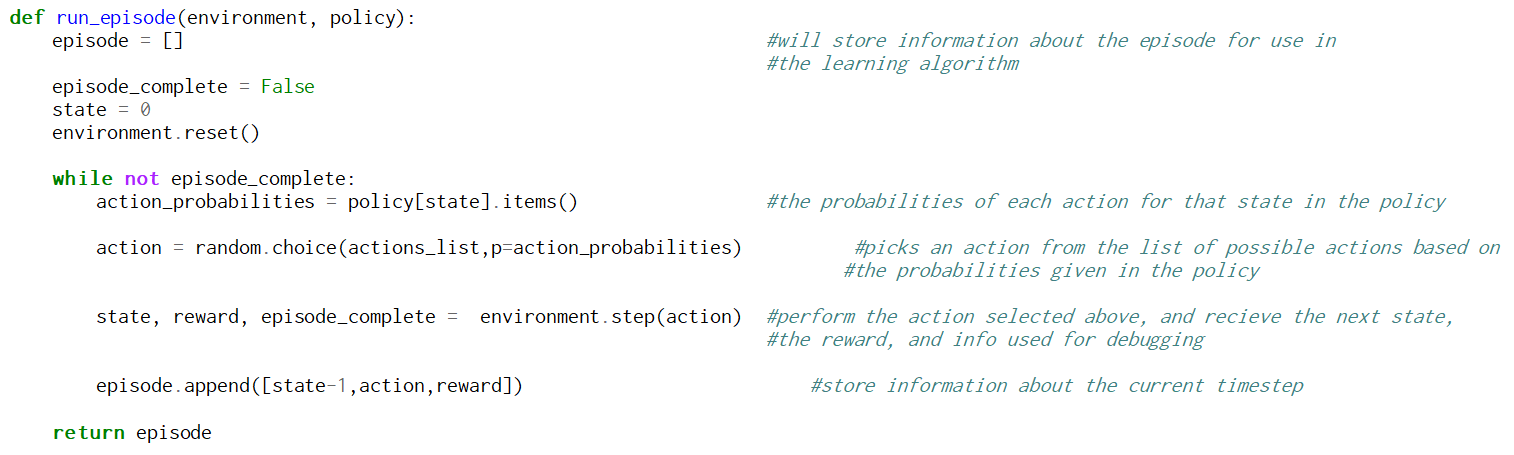
\includegraphics[width=\textwidth]{images/run}
\caption[run episode pseudocode for Monte Carlo]{pseudocode for running a single episode of an environment for the Monte Carlo algorithm}
\label{fig:mcrun}
\end{figure}

\begin{figure}[h]
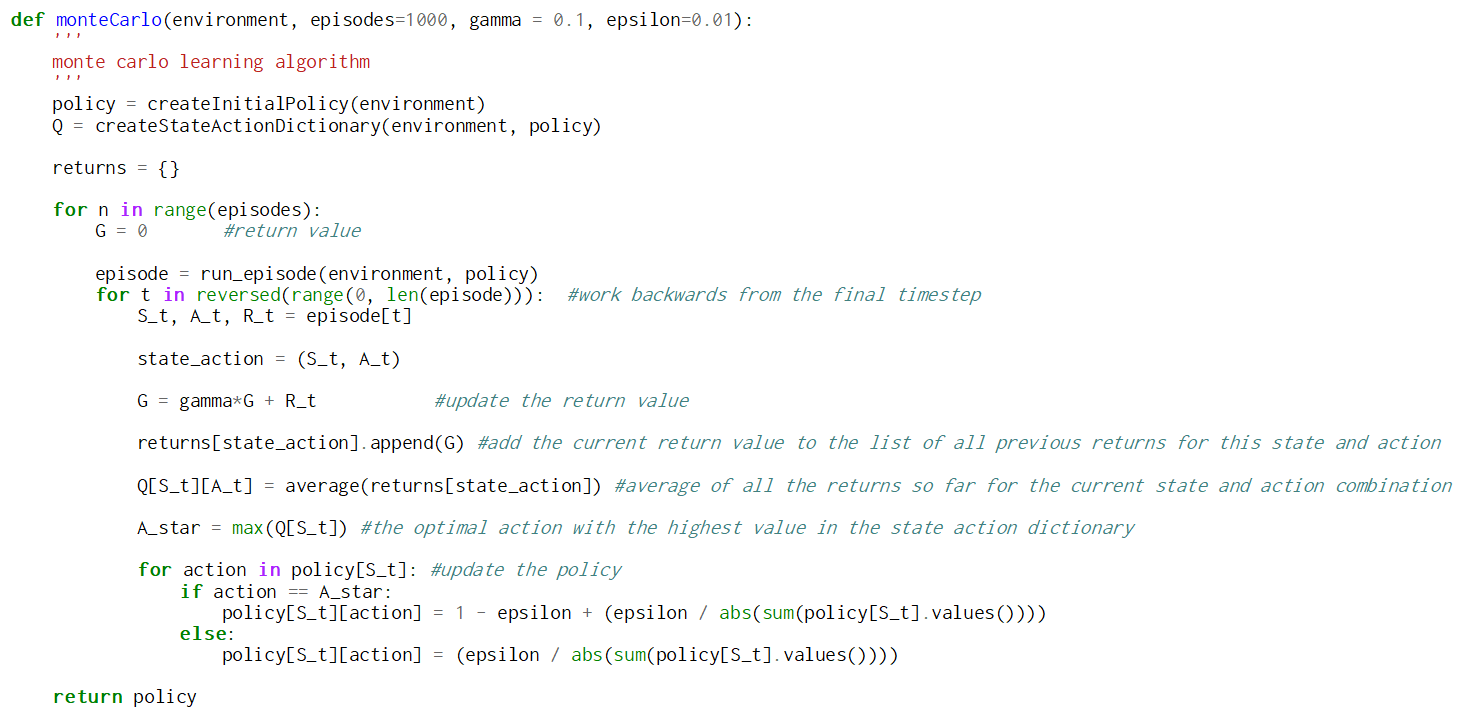
\includegraphics[width=\textwidth]{images/mcpseudo}
\caption[Monte Carlo implementation pseudocode]{pseudocode of the Monte Carlo first visit algorithm}
\label{fig:mcpseudo}
\end{figure}
Figure \ref{fig:mcrun} shows pseudocode of a basic function that runs an episode of an environment given a policy. The action is chosen based on the probabilities given within the provided policy. The state, action, and resulting reward are then stored for each timestep to be used within the Monte Carlo algorithm. Figure \ref{fig:mcpseudo} shows the pseudocode for the implementation. Note that unlike in figure \ref{fig:mcsuttonpseudo} this implementation does not have a check to see if the state has been previously visited in the episode before updating the returns list and the policy. This is due to the type of states within this environment - as each state is simply the number of operations performed, it is therefore clear that no state can be visited twice per episode, as the state will always increment with each timestep. This check can therefore be removed without affecting the underlying process.

For Q-learning, the behaviour policy (the policy used to generate data to update the reward policy) was an epsilon greedy policy, and the reward policy was a pure greedy policy. Instead of updating at the end of each episode, this policy updates after each step, as seen in figure \ref{fig:Qpseudo}.
\begin{figure}[h]
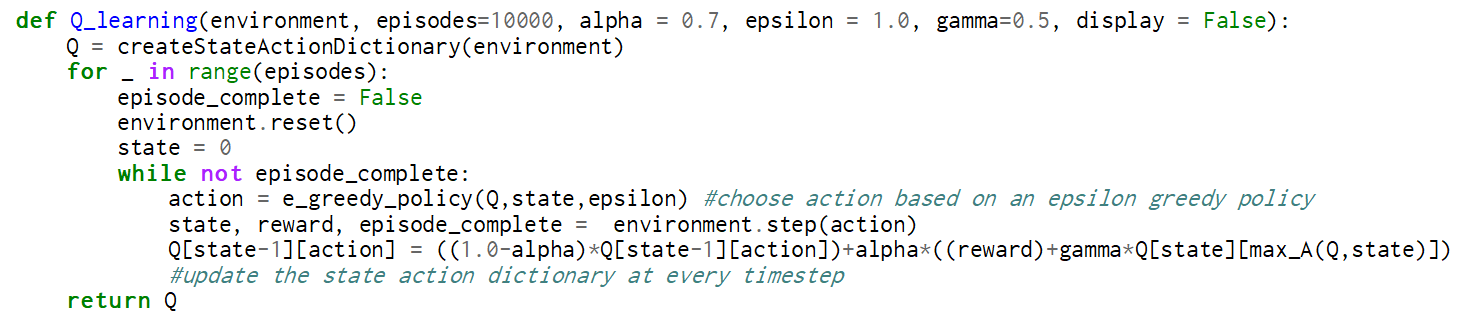
\includegraphics[width=\textwidth]{images/Qpseudo}
\caption[Q-learning implementation pseudocode]{pseudocode of the Q-learning implementation}
\label{fig:Qpseudo}
\end{figure}

